\section{Bilancio locale di potenza}
\[
 P_d = R i^2 = (\rho\frac{l}{s})|\vec J|^2 s^2 = \rho |\vec J|^2v
\]
$v$ risulta il volume del cilindro dato dalla superficie per il lato.\\
Consideriamo un volume infinitesimo centrato in un punto P. Posso definire la densità di potenza dissipata:
\[
pd(t,P) = \lim_{v\to0}\frac{P_{d,v}}{v} = \rho J^2(t,P) = \vec E_c\cdot\vec J = pe(t,P)
\]
Si usa la minuscola per la densità, per indica la densità di potenza elettrica.
\subsection{forze elettriche specifiche F.E.S generatrici}
Alcune delle FES più importanti non di natura elettrica sono la pila: di natura chimica, una turbina: di natura meccanica. Vogliamo avere la risultante delle FES: FES totale $\vec E t$ che è la somma di una parte di natura elettrica e una non elettrica. 

\section{Bilancio di potenza esteso a tutto il dominio}
Ci poniamo nell'ipotesi di conduzione stazionaria. Prendiamo $\tau_J$ volume tale in cui $\vec J \not = 0$, scriviamo il bilancio di potenza su tale volume e integriamo il bilancio di potenza locale sullo stesso.
\[\rho J^2(P) = \vec E_t(P) \cdot \vec J (P)\]
\[
\int_{\tau_J} \rho J^2dv = \int_{\tau_J} \vec E_t \cdot \vec J dv = \int_{\tau_J} \vec E_c \cdot \vec J dv + \int_{\tau_J} \vec E_g \cdot \vec Jdv
\]
Usando l'identità vettoriale:
\[
    \nabla (V\vec J) = V \nabla  (\vec J) +gradV \cdot\vec J = -\vec E_c \vec J
\]

Studiando la componente elettrica:
\[
\int_{\tau_J} \vec E_c \cdot \vec J dv = - \int_{\tau_J}\nabla(V\vec J) dv = 0
\]
Dato che $\vec E_c$ è conservativo, non compie lavoro su percorsi chiusi come sono le linee di $\vec J$. Generalmente non compie lavoro e sono necessarie FES generatrici.

\[
    \int_{\tau_J}\rho J^2dv = \int_{\tau_J}\bar Eg\cdot\bar Jdv 
\]
Risulta che la potenza dissipata (primo termine) per effetto Joule sia uguale alla potenza generata da altre forme di energia (chimica, ecc.)

Calcoliamo ora:
\[
    \int_\tau \bar Ec \cdot \bar J dv = -\int_{\partial \tau}V \bar J \cdot \hat{n}ds
\]
\[
= \cancel{\int_{sl}V \bar J \cdot \hat{n}ds} - {\int_{SA}V \bar J \cdot \hat{n}ds} - {\int_{SB}V \bar J \cdot \hat{n}ds} \not = 0
\]
\begin{center}
    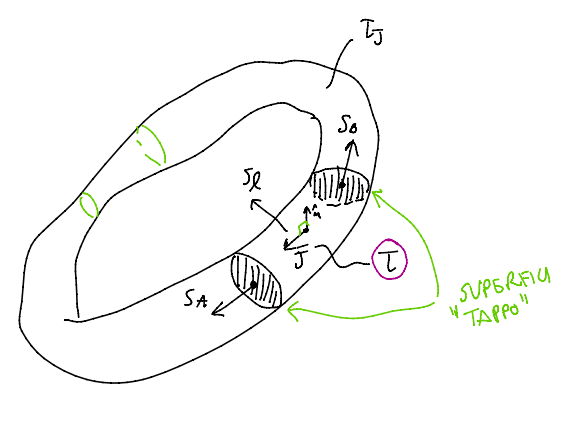
\includegraphics[scale = 0.5]{immagini/image13.png}
\end{center}
Il contributo di $\bar Ec$ su $\tau$ non è nullo. È determinante per trasferire potenza dentro $\tau_J$
\[
P_{d,\tau} = P_{g,\tau} + \int_\tau\bar Ec \cdot \bar J dv \Rightarrow P_{g,\tau} - P_{d,\tau} = - \int_\tau\bar Ec \cdot \bar J dv
\]
Risulta che la potenza dissipata è la potenza generata + la componente dell'integrale

\section{Modelli circuitali per la conduzione stazionaria}
    Modello circuitale: è una descrizione semplificata del fenomeno fisico. Per esempio nel modello di Ohm si usa solo la R in quanto interessa solo la relazione Tensione/Corrente.

    In forma generica si può calcolare la R di un conduttore. Per ipotesi si è in conduzione stazionaria ($\nabla\bar J = 0$). Consideriamo $\bar J$ tangente al bordo conduttore per canalizzazione. Questo va a denotare una porzione del tubo di flusso di $\bar J$. La corrente nel conduttore è la stessa per ogni superficie che taglia il tubo di glusso e si può quinid associare una corrente $i$ al conduttore

    \begin{center}
        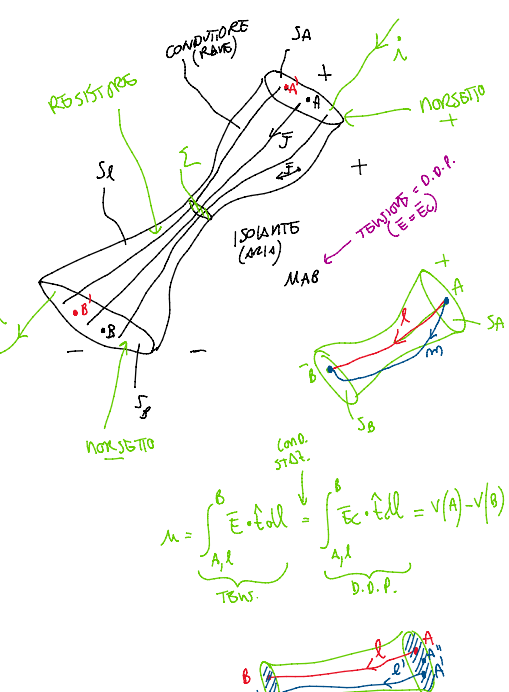
\includegraphics[scale = 0.5]{immagini/image14.png}
    \end{center}

    \subsection{Resistore}
        Ipotesi: $\bar E_t = \bar E_c$\\
        Vogliamo parlare anche di tensione ai capi del conduttore/componente. La tensione è $u = D.D.P$ in quanto regime stazionario.
        \[
            u_{AB} = \int_{A,l}^B \bar E_c \cdot\hat{t} dl
        \]
        Avere questo si deve assumere per ipotesi che $S_a$, $S_B$ siano equipotenziali. Facendo ciò si può parlare di $u$ sul componente. Si introduce la resistenza come: $R = \frac{u_{AB}}{i}$

        Con questo componente si utilizza la convenzione dell'utilizzatore: Pendo la corrente in modo che entri dal morsetto positivo.
        
        INSERIRE SCHEMI RESISTENZE

        \subsubsection{Calcolo della resistenza}
        \paragraph{Resistore filiforme}
            l è la lunghezza e si considera l>>d
            \[
            R = \frac{u}{i}
            \]
            
            \noindent
            Posso assumere $\vec{J}$ uniforme su $S$.
            
            \[
            i = \int_S \vec{J} \cdot \hat{n}\, dS = J \cdot S
            \]
            
            \noindent
            Assumendo di avere simmetria piana:
            
            \[
            u = \int_{A,l}^B \vec{E_c} \cdot \hat{t}\, dl \simeq E_C \, l = \rho J l
            \]
            \[
            \text{(Ipotesi: } |\vec{E}| \text{ uniforme)}
            \]
            
            \[
            E_c = \rho J
            \]
            
            \[
            R = \frac{u}{i} = \frac{\rho J l}{J S} = \rho \frac{l}{S} \simeq R
            \]
        \paragraph{Resistore cilindrico}
        \textbf{Simmetria cilindrica}
        \begin{center}
            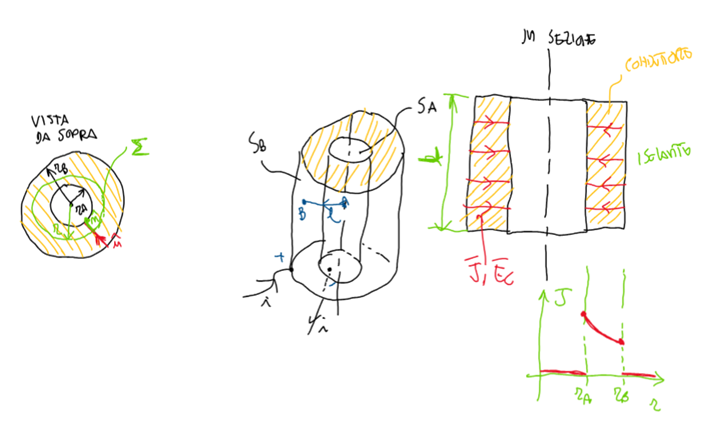
\includegraphics[scale = 0.5]{immagini/image15.png}
        \end{center}
        
        \[
        i = \int_{\Sigma} \vec{J} \cdot \hat{n}\, dS 
           = |\vec{J}| \int_{\Sigma} \hat{u} \cdot \hat{n}\, dS
           = J \Sigma = J (2 \pi r\, l)
        \]
        
        \[
        J = \frac{{i}}{2 \pi r\, l}
        \]
        
        \[
        E_c = \rho J = \frac{\rho{i}}{2 \pi r\, l}
        \]
        
        \[
        u = \int_{A,l}^{B} \vec{E_c} \cdot \hat{t}\, dl 
             = \int_{r_A}^{r_B} \frac{\rho {i}}{2 \pi r\, l}\, dr
             = \frac{\rho i}{2 \pi l} \int_{r_A}^{r_B} \frac{1}{r}\, dr
             = \frac{\rho i}{2 \pi l} \ln{\left( \frac{r_B}{r_A} \right)} = R
        \]


\paragraph{Resistore sferico}

\[
i = \int_{\Sigma} \vec{J} \cdot \hat{n}\, dS 
  = J \int_{\Sigma} \hat{u} \cdot \hat{n}\, dS 
  = J \, \Sigma 
  = J \, (4 \pi r^2)
\]

\[
J(r) = \frac{i}{4 \pi r^2}
\]

\[
E_c = \rho J = \frac{\rho \, i}{4 \pi r^2}
\]

\[
u = \int_{A,l}^{B} \vec{E_c} \cdot \hat{t}\, dl 
    = \int_{A,l}^{B} E_c \, dl 
    = \int_{r_A}^{r_B} \frac{\rho \, i}{4 \pi r^2} \, dr
\]

\[
u = \frac{\rho \, i}{4 \pi} 
       \int_{r_A}^{r_B} \frac{1}{r^2} \, dr
     = \frac{\rho \, i}{4 \pi} 
       \left( \frac{1}{r_A} - \frac{1}{r_B} \right)
\]

\[
R = \frac{u}{i} 
  = \frac{\rho}{4 \pi} 
    \left( \frac{1}{r_A} - \frac{1}{r_B} \right)
\]
1) Metà sfera\\
2) $r_B\to \infty$\\
Implica che 
\[
    R_T = \frac{\rho}{4\pi}\cdot\frac{1}{r_A}\cdot2 = \frac{\rho}{2\pi}\cdot\frac{1}{r_A}
\]
        

            